%%%%%%%%%%%%%%%%%%%%%%%%%%%%%%%%%%%%%%%%%%%%%%%%%%%%%%%%%%%%%%%%%%%%%%%%%%%%%%%%
%2345678901234567890123456789012345678901234567890123456789012345678901234567890
%        1         2         3         4         5         6         7         8

\documentclass[letterpaper, 10 pt, conference]{ieeeconf}  % Comment this line out
                                                          % if you need a4paper
%\documentclass[a4paper, 10pt, conference]{ieeeconf}      % Use this line for a4
                                                          % paper

\IEEEoverridecommandlockouts                              % This command is only
                                                          % needed if you want to
                                                          % use the \thanks command
\overrideIEEEmargins
% See the \addtolength command later in the file to balance the column lengths
% on the last page of the document




% The following packages can be found on http:\\www.ctan.org
%\usepackage{graphics} % for pdf, bitmapped graphics files
%\usepackage{epsfig} % for postscript graphics files
%\usepackage{mathptmx} % assumes new font selection scheme installed
%\usepackage{times} % assumes new font selection scheme installed
%\usepackage{amsmath} % assumes amsmath package installed
%\usepackage{amssymb}  % assumes amsmath package installed
\usepackage{csquotes}
\usepackage{graphicx}
\usepackage{url}


\title{\LARGE \bf Image Recognition and Labeling in Reduced Dimensions}
\author{David Anderton and Ray Dedhia}


\begin{document}

\maketitle
\thispagestyle{empty}
\pagestyle{empty}


%%%%%%%%%%%%%%%%%%%%%%%%%%%%%%%%%%%%%%%%%%%%%%%%%%%%%%%%%%%%%%%%%%%%%%%%%%%%%%%%

\begin{abstract}

\normalsize % increases size of font

As the use of artificial intelligence continues to expand into the realm of image compression\footnote{\url{https://ai.googleblog.com/2016/09/image-compression-with-neural-networks.html}}\footnote{\url{http://www.wave.one/icml2017/}}, questions are being raised on how well the original artefacts and nature of the source image are preserved. The consequences of being able to utilize smaller output images that maintain the majority of pertinent information from their often signifantly larger source images are huge. With smaller inputs, applications from self driving cars that rely on camera input, autonomous flight, through to training neural nets could require significantly less processing time and resources.

In this paper, we briefly examine how the Google Cloud Vision API responds to the content of a selection of images pre- and post-compression. We also consider a variety of compression techniques and extents. The goal: produce a broad estimate of how much an image can be compressed until the Google Cloud Vision API, as a proxy for other classification algorithms, can no longer determine useful insights about the constitution of the image.

An interactive exploration of the results is available at the following URI: \url{https://mit18065-dimensions.herokuapp.com/}

\end{abstract}

%%%%%%%%%%%%%%%%%%%%%%%%%%%%%%%%%%%%%%%%%%%%%%%%%%%%%%%%%%%%%%%%%%%%%%%%%%%%%%%%
\section{INTRODUCTION}

In this paper, we briefly examine how the Google Cloud Vision API responds to the content of a selection of images pre- and post-compression. We also consider a variety of compression techniques and extents. The goal: produce a broad estimate of how much an image can be compressed until the Google Cloud Vision API, as a proxy for other classification algorithms, can no longer determine useful insights about the constitution of the image.

\section{METHODOLOGY}
Our methodology was as follows:

Within our study we utilised 22 unique images, from four major
categories: six animals, six famous landmarks, five landscapes, five
street signs. Expanding this to both the color and grayscale
versions of these images, we had a resulting set of 44 source images.

After collating the source images we sent them through the Google Cloud Vision API\footnote{The Google Cloud Vision API, \url{https://cloud.google.com/vision/}, classifies images into categories and detects objects and faces in images utilising non-public machine learning models.}
and get a control set of labels for the 44 images. Then compress the images, using the five following methods:
(1) Posterization through k-means clustering,
(2) :ow-rank approximation using Principle Component Analysis (PCA),
(3) \textquote{Mean pooling} operation commonly used in neural networks,
(4) Mogrify (a command-line utility)
and (5) Dropout (randomly removing a specific percentage of the pixels).

Once the images were compressed in all of the above methods we then re-queried the Google Cloud Vision API to re-classify the images post-compression and considered the results.

\section{COMPRESSION METHODS}
\subsection{Posterization}
K-means clustering is an algorithm that groups
a set of data points into $k$ groups by mapping each data point
to one of $k$ centroids such that the distance between each data point
and its centroid is minimized. It does this by randomly generating $k$
centroids, (1) assigning each data point to the nearest centroid,
(2) updating the centroid values be setting them equal to the arithmetic
mean of the data points assigned to them in step 1, and repeating steps
1 and 2 until some stopping criteria has been met. The resulting k-means clustering implemented a posterization
effect.

We arbitrarily stopped our k-means clustering algorithm after 10 iterations as an intuitive stopping point for efficiency, and used $k=4$ and $k=8$. In figure 1 below are the results of putting an image of a cat through 4-means and 8-means clustering.

\vspace*{3mm}
\begin{tabular}{c c}
	$k=4$ & $k=8$ \\
	\includegraphics[width=0.2\textwidth]{postfour} &
		\includegraphics[width=0.2\textwidth]{posteight} \\
\end{tabular}
\begin{tabular}{l}
	{\it \hspace*{4mm} Fig. 1: Image of a cat compressed using 4-means} \\
	{\it \hspace*{4mm} and 8-means clustering.}
\end{tabular}

\subsection{PCA}
The principle components of some matrix, $M$, are its left and right singular vectors, $u_i$ and $v_i$ respectively, and its singular values,$sigma$. The decomposition of a matrix into these components is referred to most commonly as the Singular Value Decomposition, or SVD.
PCA is a form of matrix analysis that utilizes the largest principle components of a matrix of data in order to create a summarization or approximate the underlying data.

By utilising the Eckart-Young theorem\footnote{See Golub et al. \url{https://www.ime.usp.br/~jstern/miscellanea/seminario/Golub87.pdf}}, the rank $k$ matrix $M_k$ closest to $M$ is the sum of the product of the $k$ largest singular values of $M$with their corresponding left and right singular vectors. That is, $M_k = \sum_{i=1}^k \sigma_i u_i v_i^T$.

Thus, PCA can be utilised to find the best low-rank approximation for $M$.
Within our study we used PCA to reduce our image matrices to rank-5, rank-10
and rank-25 matrices. Figure 2 below shows the results of calculating the best rank-5, rank-10,
and rank-25 approximations of an image of the Tokyo Tower.

\vspace*{3mm}
\begin{tabular}{c c c}
	rank-5 & rank-10 & rank-25 \\
	\includegraphics[width=0.13\textwidth]{pcafive} &
		\includegraphics[width=0.13\textwidth]{pcaten} &
		\includegraphics[width=0.13\textwidth]{pcatwentyfive} \\
\end{tabular}
\begin{tabular}{l}
	{\it \hspace*{4mm} Fig. 2: Best rank-5, rank-10, and rank-25 matrix} \\
	{\it \hspace*{4mm} approximations of an image of the Tokyo Tower.} \\
\end{tabular}

\subsection{Mean Pooling}
Mean pooling refers to the operation of dividing
an image into regions of size $m \times n$, calculating
the arithmetic mean of those regions, and outputting
an image consisting of just those calculated averages.\footnote{See the UFLDL Tutorial on Pooling: \url{http://ufldl.stanford.edu/tutorial/supervised/Pooling/}}

For our study we considered regions of size $16 \times 16$, $32 \times 32$ and $64 \times 64$.
In figure 3 below are the results of putting an image of a US traffic light sign through
a $16 \times 16$, $32 \times 32$, and $64 \times 64$ mean pooling filter.

\vspace*{3mm}
\begin{tabular}{c c c}
	$16 \times 16$ & $32 \times 32$ & $64 \times 64$ \\
	\includegraphics[width=0.13\textwidth]{poolsixteen} &
		\includegraphics[width=0.13\textwidth]{poolthirtytwo} &
		\includegraphics[width=0.13\textwidth]{poolsixtyfour} \\
\end{tabular}
\begin{tabular}{l}
    {\it \hspace*{4mm} Fig. 3: Image of a US traffic put through $16 \times 16$,} \\
    {\it \hspace*{4mm} $32 \times 32$, and $64 \times 64$ mean pooling filters.} \\
\end{tabular}

\subsection{Mogrify}
The mogrify command line utility, part of the Image Magick suite of tools\footnote{See ImageMagick's documentation of the mogrify command: \url{https://www.imagemagick.org/script/mogrify.php}}, can be used to perform a number of operations
on images, such as blurring, cropping, and compression.
We used mogrify to compress our images using the option {\tt -quality [num]}\footnote{See ImageMagick's documentation of the quality option: \url{https://www.imagemagick.org/script/command-line-options.php\#quality}}. For JPEG image compression the expected value of {\tt [num]} is an integer from 1 to 100. We used the value of 1, that applies the most extreme JPEG compression from mogrify.
In figure 4 below, an image of the ocean before and after it has been compressed by the command {\tt mogrify -quality 1} can be considered.

\vspace*{3mm}
\begin{tabular}{c c}
	original & compressed \\
	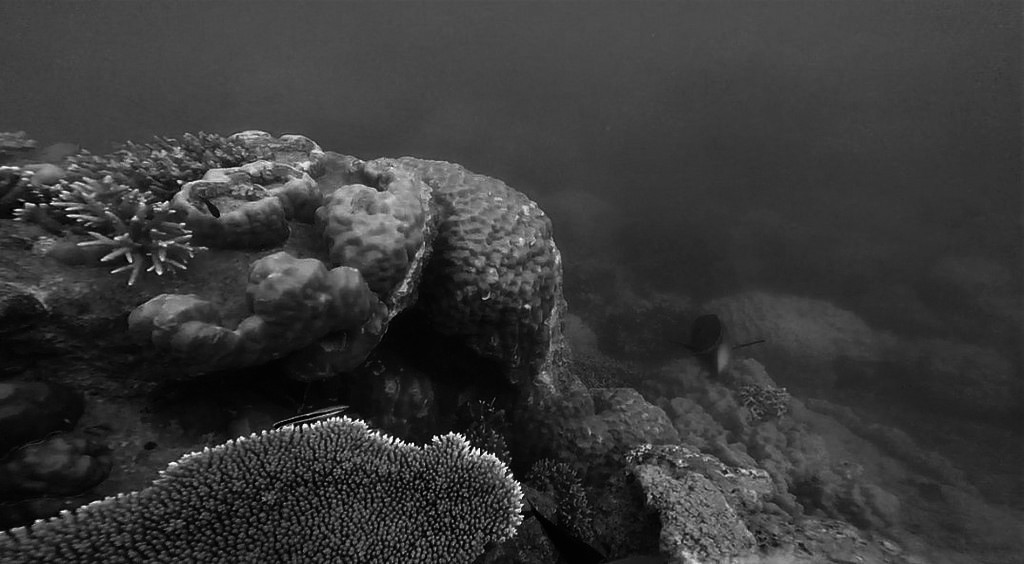
\includegraphics[width=0.2\textwidth]{ocean} &
		\includegraphics[width=0.2\textwidth]{mogrify} \\
\end{tabular}
\vspace*{3mm}
\begin{tabular}{l}
    {\it \hspace*{4mm} Fig. 4: Image of the ocean that has been compressed} \\
    {\it \hspace*{4mm} with the command {\tt mogrify -quality 1.}} \\
\end{tabular}


\subsection{Dropout}
Inspired by the concept of dropout layers in neural networks\footnote{See Srivastava et al.: \url{http://jmlr.org/papers/volume15/srivastava14a.old/srivastava14a.pdf}},
which randomly remove nodes in the neural network
to prevent overfitting, we implemented an algorithm
that randomly removes percentage $p$ of the pixels
in an image. It does this by removing
some percentage $p$ of the columns and the same percentage $p$ of the pixels
from each of the remaining columns.

We implemented this algorithm with $p=0.2,0.5$, where $p$ is a value between $0$ and $1$.
In figure 5 the results of putting an image of a tiger through dropout
with $p=0.2$ and $p=0.5$ can be considered.

\vspace*{3mm}
\begin{tabular}{c c c}
	$p=0.2$ & $p=0.5$ \\
	\includegraphics[width=0.2\textwidth]{dropouttwenty} &
		\includegraphics[width=0.2\textwidth]{dropoutfifty} \\
\end{tabular}
\begin{tabular}{l}
    {\it \hspace*{4mm} Fig. 5: Image of a tiger put through dropout with} \\
    {\it \hspace*{4mm} with $p=0.2, 0.4$.} \\
\end{tabular}


\vspace*{3mm}

\section{RESULTS}

\subsection{Pre-Compression}

Once the collection of images in the various categories had been located through Creative Commons Image Search\footnote{See: https://search.creativecommons.org/} the images were then sent via http request to the Google Cloud Vision API and returned with an assigned set of labels and respective confidence score.
All of the labels assigned to the color images were
found to be intuitively accurate and relevant by the authors, and for each color image,
at least one label closely identified the image (e.g. \textquote{tiger}
for the iamge of a tiger and \textquote{tower} for the image of
the Tokyo Tower).

However, not all the grayscale versions of images were accurately classified according to the authors intuition.
Generic labels such as \textquote{black and white}, \textquote{black}, \textquote{white}, \textquote{art},
and \textquote{monochrome photography} were prevalent throughout greyscale images - a behavior noted later in this paper where the artefacts of compression were noted as an classifiable part of the image. According to the authors judgement 40.9\% of the grayscale images
were not closely identified, and 18.2\% of them were given solely inaccurate labels.

\subsection{Post-Compression}

Table 1 and 2 below display our analysis of how accurately images are labeled by the
Google Cloud Vision API after they are compressed using each
the methods detailed earlier in the paper. We define accuracy as the coincidence of labels between pre- and post-compression images.  We ignored more general
labels such as \textquote{photography,} \textquote{black,}
and \textquote{sky,} instead focusing on labels that either correctly or falsely
identify specific objects, landforms, etc. in the images.

\vspace*{2mm}

\hspace*{28mm} \underline{Color Images}

\vspace*{2mm}

\bgroup
\def\arraystretch{1.2} % stretches table vertically
\begin{tabular}{|p{0.25\linewidth}|p{0.25\linewidth}|p{0.25\linewidth}|}
\hline
{\bf method of compression} & {\bf \% images given at least one correct label}
	& {\bf \% images given "best" label} \\
\hline
Mogrify & 81.8\% & 68.2\% \\ % 18/22, 15/22
\hline
Dropout (20\%) & 77.3\% & 68.2\% \\ % 7/22, 15/22
\hline
Dropout (50\%) & 59.1\% & 36.4\% \\ % 13/22, 8/22
\hline
Pooling (16x16) & 90.9\% & 63.6\% \\ % 20/22, 14/22
\hline
Pooling (32x32) & 40.9\% & 18.2\% \\ % 9/22, 4/22
\hline
Pooling (64x64) & 4.5\% & 0\% \\ % 1/22, 0/22
\hline
PCA (25) & 95.5\% & 81.8\% \\ % 21/22, 18/22
\hline
PCA (10) & 77.3\% & 40.9\% \\ % 17/22, 9/22
\hline
PCA (5) & 27.3\% & 0\% \\ % 6/22, 0/22
\hline
Clustering (8) & 100\% & 90.9\% \\ % 22/22, 20/22
\hline
Clustering (4) & 86.4\% & 68.2\% \\ % 19/22, 15/22
\hline
\end{tabular}
\egroup

\vspace*{2mm}
\begin{tabular}{l}
{\it Table 1: Success rate for color images} \\
{\it labeled by Google Cloud Vision API after} \\
{\it image compression.} \\
\end{tabular}
\vspace*{4mm}

\vspace*{2mm}

\hspace*{28mm} \underline{Grayscale Images}

\vspace*{2mm}

\bgroup
\def\arraystretch{1.2} % stretches table vertically
\begin{tabular}{|p{0.25\linewidth}|p{0.25\linewidth}|p{0.25\linewidth}|}
\hline
{\bf method of compression} & {\bf \% images given at least one correct label}
	& {\bf \% images given best label} \\
\hline
Mogrify & 59.1\% & 40.9\% \\ % updated
\hline
Dropout (20\%) & 63.6\% & 27.3\% \\ % updated 14/22, 6/22
\hline
Dropout (50\%) & 22.7\% & 0\% \\ % updated 5/22, 0/22
\hline
Pooling (16x16) & 31.8\% & 22.7\% \\ % updated 7/22, 5/22
\hline
Pooling (32x32) & 4.5\% & 4.5\%\\ % updated 1/22, 1/22
\hline
Pooling (64x64) & 0\% & 0\% \\ % updated 0, 0
\hline
PCA (25) & 68.2\% & 36.4\% \\ % updated 15/22, 8/22
\hline
PCA (10) & 31.8\% & 22.7\% \\ % updated 7/22, 5/22
\hline
PCA (5) & 18.2\% & 4.5\% \\ % updated 4/22, 1/22
\hline
Clustering (8) & 90.9\% & 50\% \\ % updated 20/22, 11/22
\hline
Clustering (4) & 59.1\% & 45.5\% \\ % updated 13/22, 10/22
\hline
\end{tabular}
\egroup

\vspace*{2mm}
\begin{tabular}{l}
{\it Table 2: Success rate for grayscale images} \\
{\it labeled by Google Cloud Vision API after} \\
{\it image compression.} \\
\end{tabular}

\def\arraystretch{1.0} % removes vertical stretch

\vspace*{4mm}

\section{ANALYSIS}

As expected, the less the image was compressed, the more accurate
the labels it was assigned were. The grayscale images were also
given significantly less accurate labels than the color images.
Of the four categories, the animal dataset had the best
performance, most likely because the animal images had only
one subject, making them easier for Google Cloud Vision API to classify.
In addition, each form of image
compression had its own set of issues.

The smoothening effect of posterization using the k-means clustering
algorithm sometimes removed textures that Google Cloud Vision API
needed to correctly classify parts of an image. For instance,
the image of the waterfall, after it was put through the
4-means and 8-means clustering algorithm, was assigned the label \textquote{snow}
by Google Cloud Vision API because the Google Cloud Vision API mistook
the smoothened water for snow (see Fig. 6 below).

\vspace*{3mm}
\begin{tabular}{c c}
	original & compressed ($k=8$) \\
	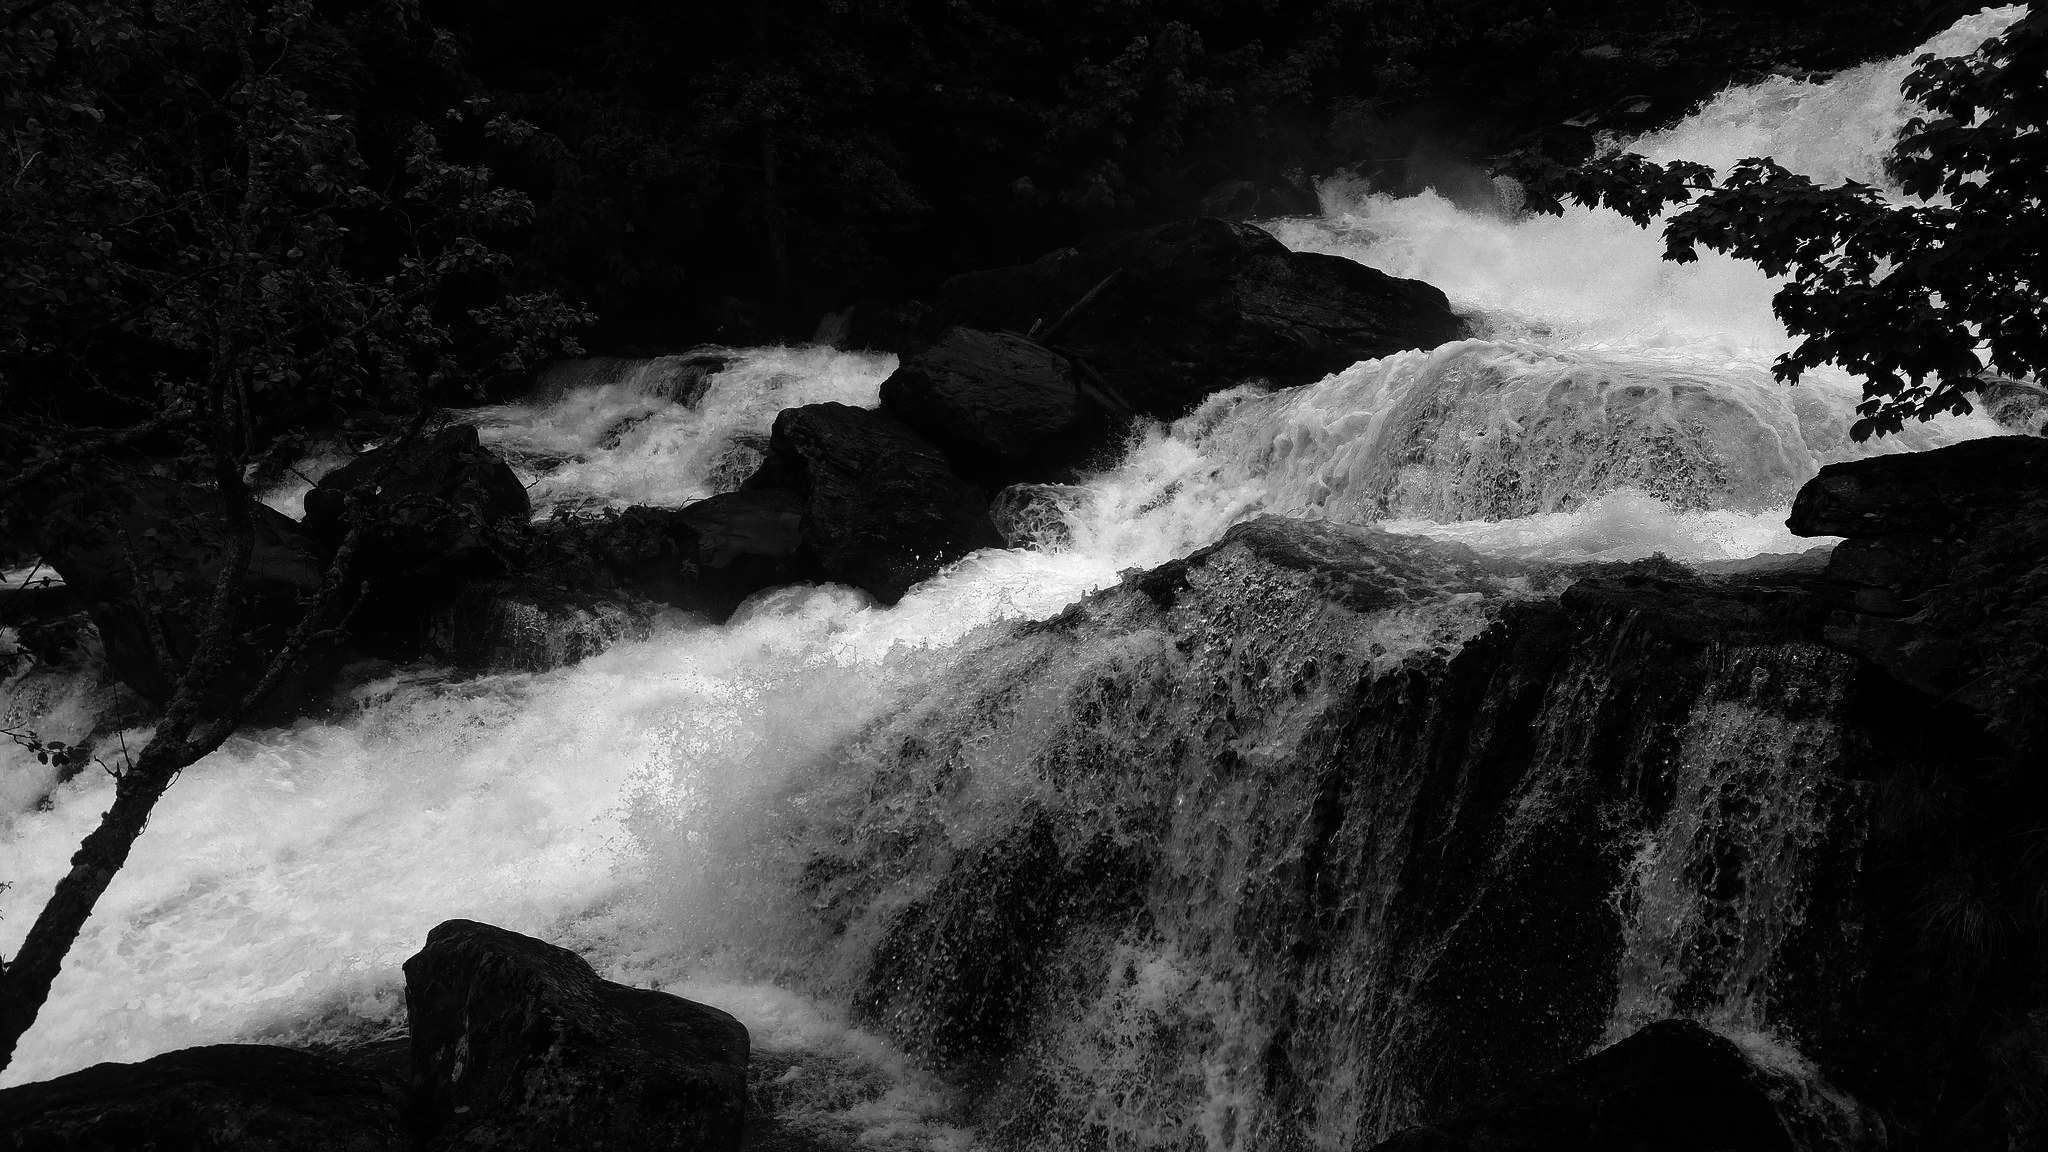
\includegraphics[width=0.2\textwidth]{waterfall} &
		\includegraphics[width=0.2\textwidth]{posterror} \\
\end{tabular}
\begin{tabular}{l}
	\hspace*{4mm} {\it Fig. 6: Over-smoothening of an image of a waterfall} \\
	\hspace*{4mm} {\it as a result of the 8-means clustering algorithm.} \\
\end{tabular}
\vspace*{3mm}

Low-rank image matrix approximation using PCA often resulted in
image distortion in a plaid-like pattern, especially in smaller
images (see Fig. 7 below). This resulted in misclassifications
such as Google Cloud Vision API giving images in all four categories
false labels such as \textquote{cloth,} \textquote{pattern,}
and \textquote{line.}

\vspace*{3mm}
\begin{tabular}{c c}
	original & rank-5 \\
	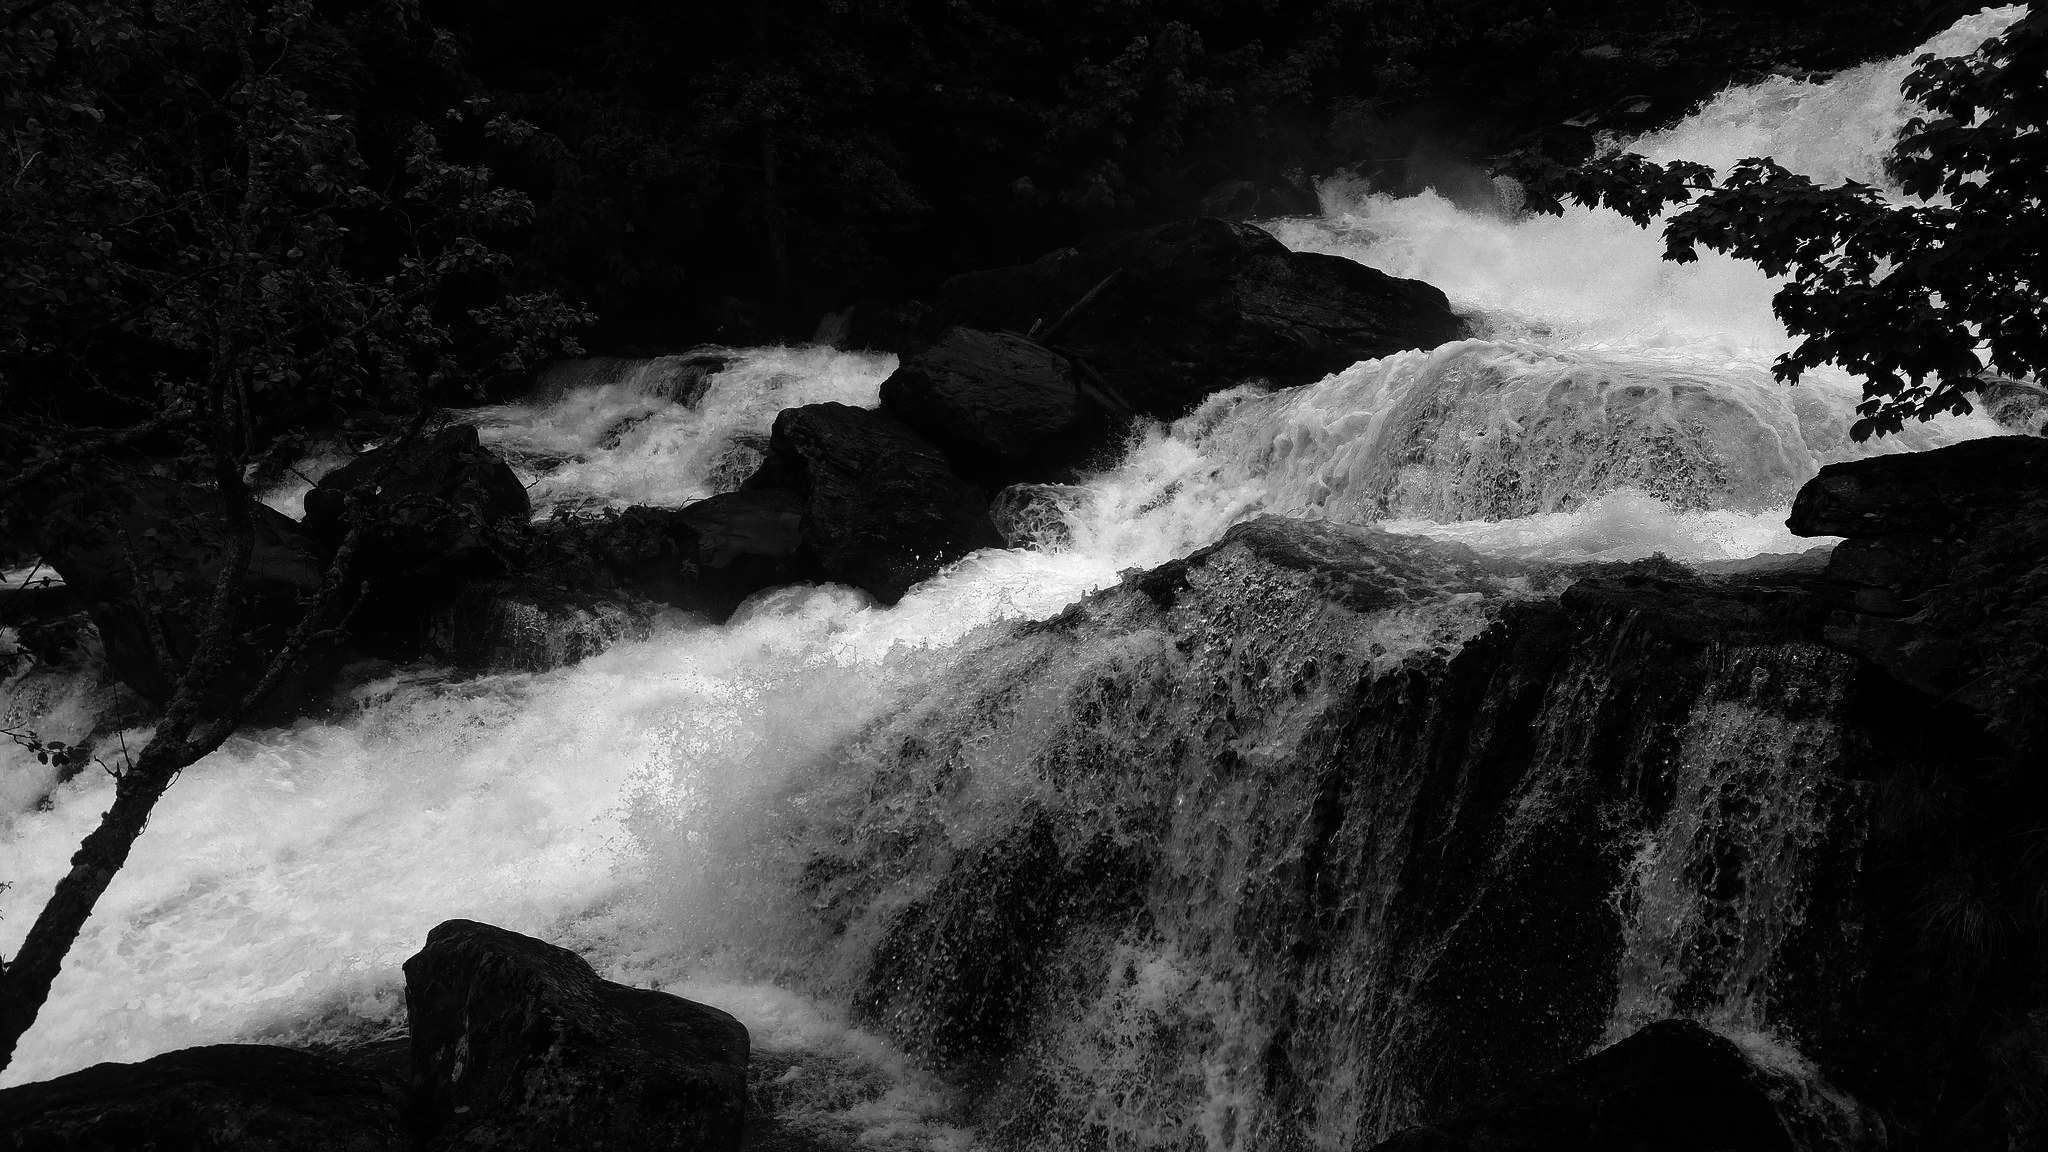
\includegraphics[width=0.2\textwidth]{waterfall} &
		\includegraphics[width=0.2\textwidth]{pcafiveerror} \\
\end{tabular}

\begin{tabular}{c c}
	rank-10 & rank-25 \\
	\includegraphics[width=0.2\textwidth]{pcatenerror} &
		\includegraphics[width=0.2\textwidth]{pcatwentyfiveerror} \\
\end{tabular}
\begin{tabular}{l}
	\hspace*{4mm} {\it Fig. 7: Distortions in the low-rank matrix } \\
	\hspace*{4mm} {\it approximations of an image of a waterfall.} \\
\end{tabular}
\vspace*{3mm}

The \textquote{mean pooling} opeartion with a $64 \times 64$ filter,
and, in some cases, the $32 \times 32$ filter as well,
blurred smaller to the point that they become unrecognizeable and
Google Cloud Vision API could no longer give them accurate labels (see
Fig. 3). When the filter being used with the \textquote{mean pooling}
operation is too large proportional to the size of the image, it
removes all useful information from the image.

Image compression using the {\tt mogrify -quality 1} command
sometimes resulted in random bright colors showing up in the compressed
images that did not occur in the original images (see Fig. 8 below).

\vspace*{3mm}
\begin{tabular}{c c}
	original & compressed \\
	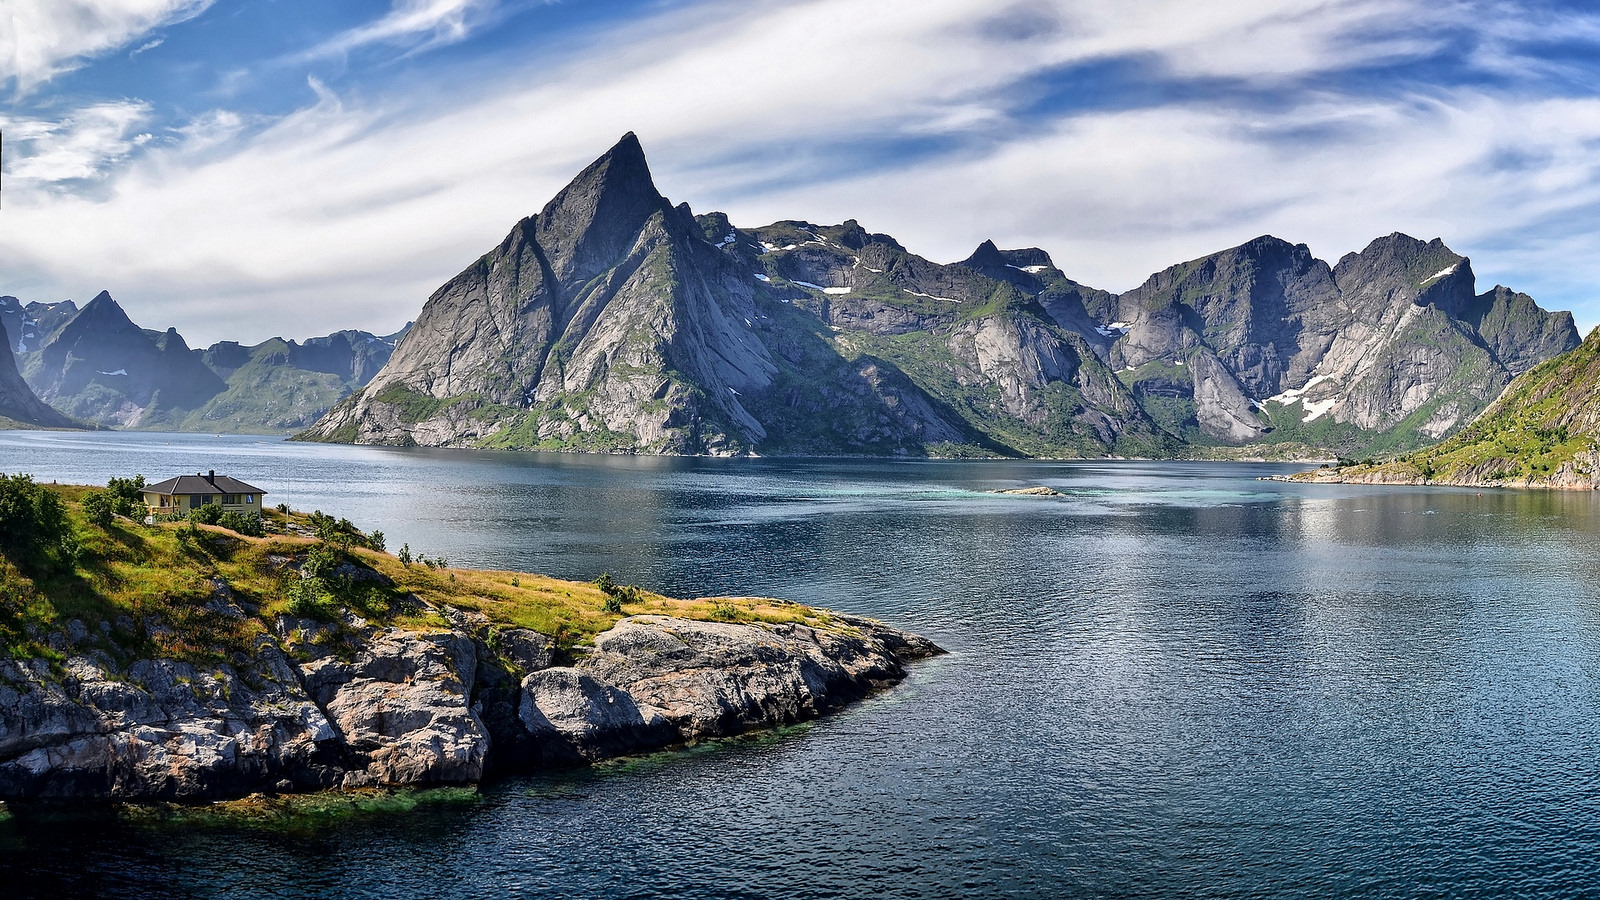
\includegraphics[width=0.2\textwidth]{mountains} &
		\includegraphics[width=0.2\textwidth]{mogrifyerror} \\
\end{tabular}
\begin{tabular}{l}
	\hspace*{4mm} {\it Fig. 8: Purple highlights appear in an image of } \\
	\hspace*{4mm} {\it mountains after it is compressed using the } \\
	\hspace*{4mm} {\it command} {\tt mogrify -quality 1} \\
\end{tabular}
\vspace*{3mm}

The dropout algorithm we created resulted in distortion of
the compressed images, almost as though the images
were being reflected on moving water.
This could potentially be fixed by adding a smoothening
factor to our dropout algorithm, for example by
using an algorithm such as seam-carving\footnote{For a description
of seam-carving, see: \url{https://cs.brown.edu/courses/cs129/results/proj3/taox/}}

\section{CONCLUSION}

Overall, from the data, it appears that k-means clustering was
the best compression method in terms of maintaining the legibility
of the images for Google Cloud Vision API. In a sense, this makes
sense, because posterization generally simplifies images while
retaining the overall shapes in the images.

Users would most likely want to use at least 8-means clustering
to reduce the dimensionality of their data.
If there data is larger than the images that we studied in this paper,
they will probably want to use even higher values of $k$.

\section{FUTURE RESEARCH}

In future analyses, it may be helpful to estalish a more
specific definition of accuracy and a way to compare
the accuracy of Google Cloud Vision API when classifying
images before and after compression, as the table
above does not consider a number of factors, such as
the certainty of different labels, and the number
of completely incorrect labels assigned to images.

In addition, we can explore the ways in which the different
image compression methods we investigated in this paper
could be used to combat adversarial attacks, in which
stickers, random noise, etc. are added to images, causing
neural networks to miscassify them or fail to detect them
\footnote{\url{https://openreview.net/pdf?id=S10qYwywf}},
as research has shown that data reduction can be used a method to fight
adversarial attacks.\footnote{\url{https://www.researchgate.net/publication/315890594\_Dimensionality\_Reduction\_as\_a\_Defense\_against\_Evasion\_Attacks\_on\_Machine\_ Learning\_Classifiers}}

% Extra example removed
%For exmaple, putting adversarial stickers on stop signs
%can cause neural networks to be unable to detect stop signs.\footnote{\url{http://bair.berkeley.edu/blog/2017/12/30/yolo-attack/}}

\addtolength{\textheight}{-12cm}   % This command serves to balance the column lengths
                                  % on the last page of the document manually. It shortens
                                  % the textheight of the last page by a suitable amount.
                                  % This command does not take effect until the next page
                                  % so it should come on the page before the last. Make
                                  % sure that you do not shorten the textheight too much.

%%%%%%%%%%%%%%%%%%%%%%%%%%%%%%%%%%%%%%%%%%%%%%%%%%%%%%%%%%%%%%%%%%%%%%%%%%%%%%%%

\section*{ACKNOWLEDGMENT}

We would like to thank Prof. Strang for his support and interesting and informative lectures.

%%%%%%%%%%%%%%%%%%%%%%%%%%%%%%%%%%%%%%%%%%%%%%%%%%%%%%%%%%%%%%%%%%%%%%%%%%%%%%%%
\begin{thebibliography}{99}

\bibitem{c1} Johnston, Nick and David Minnen. \textquote{Image Compression With Neural Networks.} Google AI Blog. Published 29 September 2016. \url{https://ai.googleblog.com/2016/09/image-compression-with-neural-networks.html}
\bibitem{c2} \textquote{Real-Time Adaptive Image Compression.} WaveOne, Inc. WaveOne. Published May 2017. \url{http://www.wave.one/icml2017/}
\bibitem{c3} \textquote{Cloud Vision API.} Google Cloud. \url{https://cloud.google.com/vision/}
\bibitem{c4} Golub, G. H., Alan Hoffman and G. W. Stewart. \textquote{A Generalization of the
	Eckart-Young-Mirsky Matrix Approximation Theorem.} \url{https://www.ime.usp.br/~jstern/miscellanea/seminario/Golub87.pdf}
\bibitem{c5} \textquote{Pooling.} UFLDL Tutorial. \url{http://ufldl.stanford.edu/tutorial/supervised/Pooling/}
\bibitem{c6} \textquote{mogrify.} ImageMagick. \url{https://www.imagemagick.org/script/mogrify.php}
\bibitem{c7} \textquote{command line options.} ImageMagick. \url{https://www.imagemagick.org/script/command-line-options.php\#quality}
\bibitem{c8} Srivastava, Nitish, et. al. \textquote{Dropout: A Simple Way to Prevent Neural Networks
	from Overfitting.} {\it Journal of Machine Learning Research}, 15 (2014): 1929-1958.
	Published 14 June 2014. \url{http://jmlr.org/papers/volume15/srivastava14a.old/srivastava14a.pdf}
\bibitem{c9} Tao, Xiaofeng. \textquote{Seam Carving.} \url{https://cs.brown.edu/courses/cs129/results/proj3/taox/}
\bibitem{c10} Gopalakrishnan, Soorya, et. al. \textquote{Combating Adversarial
	Attacks Using Sparse Representations.} ICLR 2018. \url{https://openreview.net/pdf?id=S10qYwywf}
\bibitem{c11} Bhagoji, Arjun, et. al. \textquote{Dimensionality Reduction as a Defense against Evasion Attacks on Machine Learning Classifiers.} \url{https://www.researchgate.net/publication/315890594\_Dimensionality\_Reduction\_as\_a\_Defense\_against\_Evasion\_Attacks\_on\_Machine\_ Learning\_Classifiers}
\bibitem{c12} Evtimov, Ivan, et. al. \textquote{Physical Adversarial Examples Against Deep
	Learning Networks.} Berkeley Artificial Intelligence Research. Published 30 December 2017. \url{http://bair.berkeley.edu/blog/2017/12/30/yolo-attack/}

\end{thebibliography}

\end{document}
